\begin{proof}
    We have to use \textbf{averaged} uniform stab (this is a randomized algo!)
\end{proof}





\item For $ T \geq n $ (multipasses over the data) with rempalcement, Lemma 1 of this lecture give 
\begin{align*}
    \mathcal{R}(A(\mathcal{D}_n, T)) - \mathcal{R}^\star 
        &\leq \underbrace{\beta (n,T)}_{\text{stability}} + \underbrace{Optim(T \text{ iter})}_{Optimisation} \\
        &\leq \underbrace{\frac{2 \beta ^2 R^2}{n }\sum_{}^{}\gamma _t}_{\text{Today}} + \underbrace{\frac{\left\| \theta _0 - \theta ^\star  \right\| }{\gamma T } + \gamma \sigma ^2}_{\text{with } \gamma \text{ cst (cf previus lecture)} }
\end{align*}
\textbf{Good}: We have obtained a generalization bound for nay nb $ T $ of iteration \\
\textbf{Trade-off} between stability and optimisation. This suggest the existence of an optimal "EARLY STOPPING" time $ T^\star  $, such that the risk decreases up to $ T^\star  $ 

\begin{figure}[!h]
    \centering
    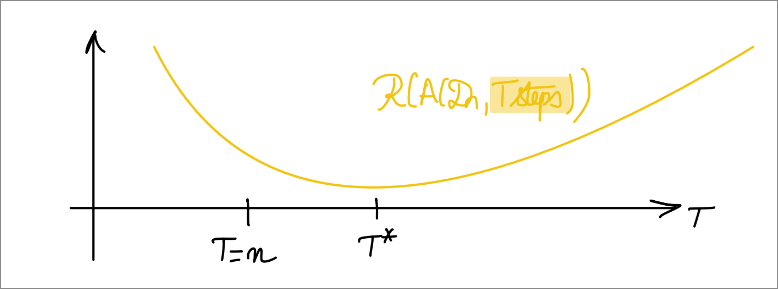
\includegraphics[width=.75\textwidth]{figs/early_stoping.png}
    \caption{Early Stopping}
\end{figure}

